\title{Evaluating Performance Characteristic of Opportunistic Routing Protocols in ONE}
\author{
  G54ACN\\
  Jack Ellis\\
  psyje5@nottingham.ac.uk\\
  4262333
}
\date{}
\documentclass[12pt]{report}
\usepackage{graphicx}
\graphicspath{ {./Images/} }
\usepackage{mathtools}
\usepackage{listings}
\lstset{
  basicstyle=\ttfamily\small,
  xleftmargin=-0.1\textwidth,
  xrightmargin=-0.1\textwidth
}

\begin{document}
\maketitle
\tableofcontents
\pagebreak

\section{Describing Opportunistic Networks and the ONE Simulator}
\subsection{Opportunistic Networks}

An opportunistic network is a term used to describe a network in which nodes communicate with one another by way of "hopping" between other nodes, as opposed to a more traditional "static" network structure in which traffic is sent through, and organised by, a central router.
Nodes can be any device with the ability to recieve or transmit data to/from its neighbour, typically via Bluetooth, Wi-Fi, or 3G/4G.
These nodes act as clients, servers, and routers all at once to forward packets (sometimes their own) from source to destination, and may come with constraints on buffer size, bandwidth, computational resources, power, and so on.
The topology of these networks is not fixed, and changes frequently and unpredictably, however this is not to say such networks cannot make use of static points to augment the nodes present on the network.

\par

In this setup there can be no assumption of the existence of a complete path from sender (\textit{S}) to recipient (\textit{R}).
Those two nodes might never be connected to the same network at the same time, and consequently techniques must be used to ensure that if \textit{S} sends a message it can "wait" on the network until such a time as \textit{R} is available and can recieve it.
This often comes at a cost: an additional delay in message delivery, due to the fact that messages are often buffered in the network waiting for a path to become available.

\par

Returning to the "node hops" idea, the way in which these hops are determined depends upon the protocol chosen for the network.
Routes are calculated at each hop, so each node will make use of local knowledge to determine the best "next hop", based on what it knows about its immediate neighbours, to make so the message can reach its intended destination.
If no good hop exists (which is to say that no other nodes are in range or the neighbours are considered unsuitable), the node can store the message and wait while future opportunities arise for forwarding.
This technique is, somewhat unsurprisingly, called "store and carry forward".

\subsubsection{Opportunistic Networks vs MANETs, VANETs, and DTNs}
Mobile Ad-hoc NETworks (MANETs), Vehicular Ad-hoc NETworks (VANETs), and Delay-Tolerant Networks (DTNs) all appear as types of opportunistic network, however in most cases they are not.

DTNs are generally regarded as a subset of opportunistic network, and the most extreme cases thereof\cite{ieeemag}.
The key difference here is that DTNs assume certain things about the network, such as the idea that some links could only be available at certain times, opportunistic networks don't require any knowledge of the network whatsoever.
This difference leads to the fact that routes in DTNs are precomputed by taking into account planned unavailability, whereas routes in opportunistic networks are computed at each hop (as described above).

\par

MANETs and VANETs require knowledge of the network's topology, routing protocols used within them need to know the layout of the network in order to function, as opposed to a true opportunistic network, which only cares about the "next hop".

\subsection{The ONE Simulator}

The Opportunistic Network Environment (ONE) Simulator is a network simulator built in Java and capable of:

\begin{center}
  \begin{itemize}
    \item \textit{Generating node movement using different movement models}
    \item \textit{Routing messages between nodes with various DTN routing algorithms and sender and receiver types}
    \item \textit{Visualizing both mobility and message passing in real time in its graphical user interface.}
    \item \textit{ONE can import mobility data from real-world traces or other mobility generators. It can also produce a variety of reports from node movement to message passing and general statistics.}\cite{onewebsite}
  \end{itemize}
\end{center}

This means that it can simulate network activity, based on a network map and protocols.
In Figure \ref{fig:oneoverview}, we can see the basic elements of ONE, as well as how they interact with one another\cite{simutools}.

\begin{figure}[ht]
  \caption{An overview of the ONE Simulator}
  \centering
  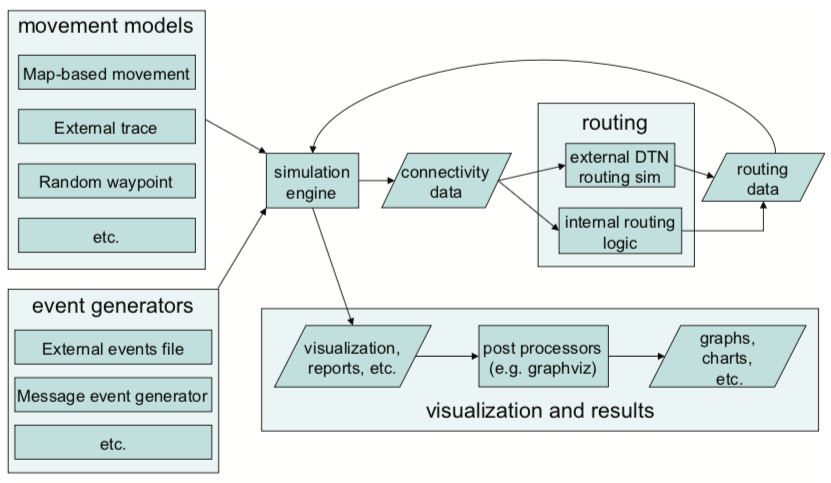
\includegraphics[width=0.5\textwidth]{ONEOverview.png}
  \label{fig:oneoverview}
\end{figure}

A potential drawback of the ONE simulator is the fact that it only supports 6 routing protocols by default\cite{simutools}.
This however is mitigated by the fact that all of these protocols take the form of Java source files, meaning a user can define any number of custom protocols, or modify the extant ones as they see fit.

\begin{figure}[ht]
  \caption{A screenshot of ONE running its default scenario, on a map of the Finnish capital Helsinki}
  \centering
  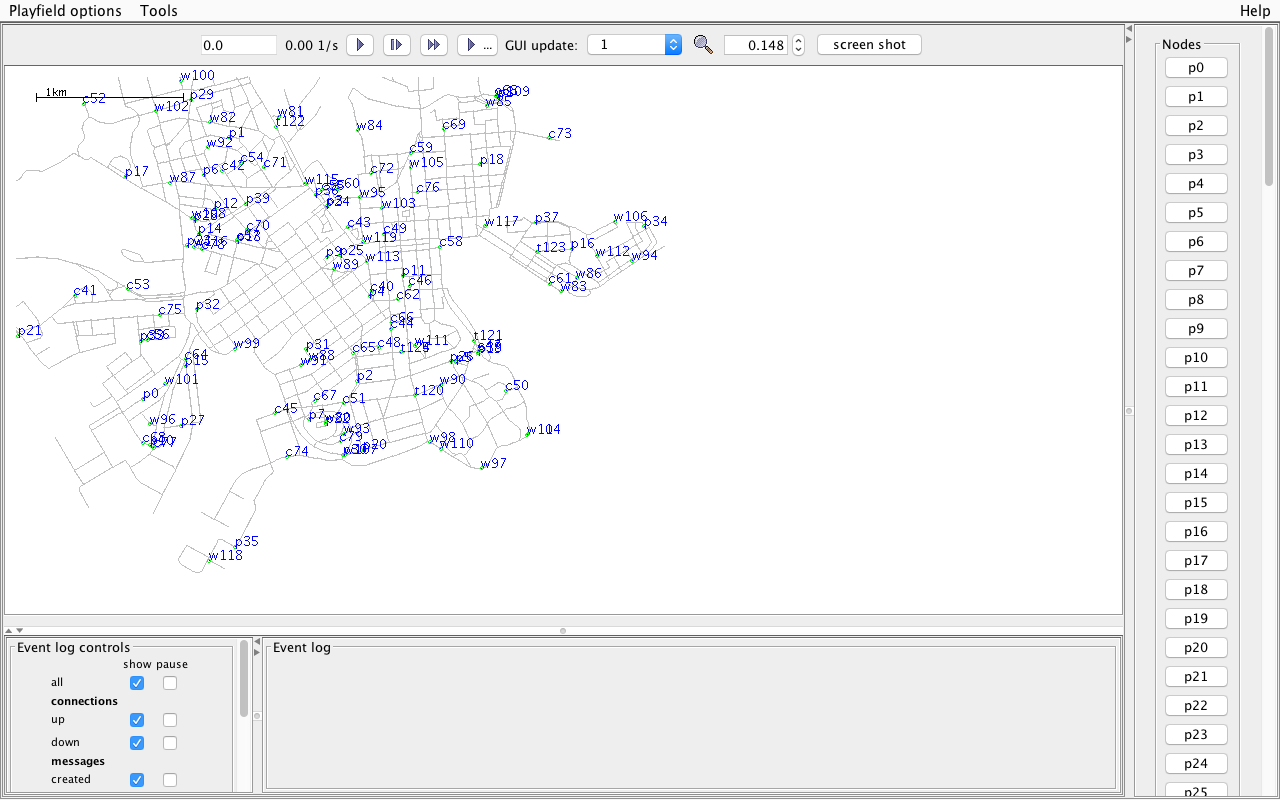
\includegraphics[width=0.5\textwidth]{ONEScreenshot.png}
  \label{fig:onescreenshot}
\end{figure}

Figure \ref{fig:onescreenshot} shows the ONE simulator's GUI in its default state.
If a user clicks on a node from this view they are given a more detailed overview of that node; as an example I selected node \verb|p12| and let the simulator run for a few seconds.
Figure \ref{fig:oneeventlog} shows the event log generated by this.

\begin{figure}[ht]
  \caption{A screenshot of ONE's event log showing a node's connection history}
  \centering
  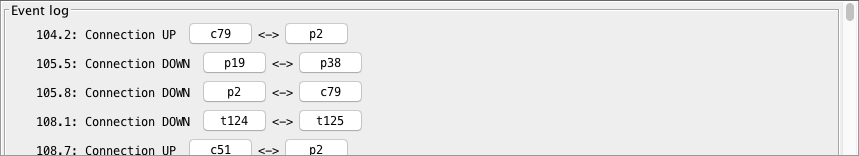
\includegraphics[width=0.5\textwidth]{ONEEventLog.png}
  \label{fig:oneeventlog}
\end{figure}

ONE can also be used in what is known as "batch mode" to simulate and generate reports for a wide range of scenarios.
To do this on a Mac, one must navigate to ONE's directory and, assuming it is compiled properly, run the following command.

\begin{lstlisting}
./one.sh -b n
\end{lstlisting}

Where \verb|n| is the number of times you want the program to run.
As seen later the settings file for ONE can be non-deterministic; this is to say that it can have multiple options (hereafter arrays) with regards to settings for a particular parameter.
A drawback here - or at least something a user should be aware of - is that the simulator will "walk through" each array in lock-step; selecting on the first run the first value of each array, the second run the second value of each array, and so on.
The consequence of this is that no two parameters' arrays should have lengths with the same lowest common factor (unless these values must change similarly).

\section{Choosing two Opportunistic DTN protocols}
I have selected two replication-based protocols for my study, in the main because they are both commonly used benchmark protocols.

\subsection{Protocol 1: Probabilistic Routing Protocol using History of Encounters and Transitivity (Prophet)}
Prophet is a replication-based protocol that keeps track of which nodes a message has encountered by way of a vector.
This vector is used to calculate the probability of a message copy finding the destination by being forwarded to a particular node.
This heuristical approach does mean that a training period is required in order to find the initial probabilities.
\par
When a source node forwards a copy of the message, it chooses a subset of possible target nodes.
These nodes are then ranked based on the calculated probabilities, with the copy being forwarded to the highest-ranked node.\cite{prophetreport1}
While this is effective, the routing tables grow incredibly quickly as a consquence of the amount of node information needed for the probability calculations, and again, this "training period" means it will take time for the algorithm to become truly effective.

\subsection{Protocol 2: Epidemic}
Epidemic\cite{epidemicreport} is one of the earlies and most simple replication-based approach to sending messages.
It utilises the concept of flooding, i.e. it attempts to ensure the message is recieved by sending it to every possible node on the network.
When two nodes meet they compare what messages they have stored; they then exchange copies that they do not have in common.
This is repeated across all node pairs on the network, spreading the message through the network like a disease epidemic, hence the name.
\par
While this method can achieve low latency and high delivery success rate, it does not take into account (and therefore suffers from) the problem of limited resources that all replication-based schemes suffer from.
This is to say that a large amount of resources are consumed by the approach, mainly buffer space, an issue often made worse by the fact that redundant copies of messages are often left on the network after a successful delivery.
Some efforts have been made to mitigate this, sending a "vaccine" message to a node to indicate that a stored message may be discarded\cite{vaccines}.

\section{Description of Experiment Setup and Scenario}

The experiment will involve comparing both protocols' performance response to different numbers of nodes and different message sizes.
The basic scenario is a disaster in the Finnish city of Helsinki; some event has rendered public transport useless and pedestrians and car drivers are messaging each other to determine what has happened.
The increasing message sizes will represent the move between simple text messages, through photographs and finally video files being shared about their situation.
Hence there will be a total of 10 message sizes:
\begin{itemize}
  \item 500 kilobytes
  \item 1 megabyte
  \item 1.5 megabytes
  \item 2 megabytes
  \item 2.5 megabytes
  \item 3 megabyte
  \item 3.5 megabytes
  \item 4 megabytes
  \item 4.5 megabytes
  \item 5 megabytes
\end{itemize}

The number of nodes will represent the number of people who either notice or are awake at the time (this can be thought of as simulating different times of day as fewer people will be awake at night), and will range in steps of 10 from 40 to 100, in two groups: people and cars.

\par

These two groups will represent pedestrians who will message one another about the event occuring, and taxicab drivers who will be relaying information about roads to avoid, problem areas, etc.
In this scenario delivery probability and latency are the key metrics: delivery probability because a message is useless if it does not get to where it needs to go, and latency because a delivered message is useless if it is too late to act upon its contents.
Additionally to these metrics, there are a number of other interesting metrics we can observe; hop count can be tied to latency to tell us how a differing number of hops required can change the time it will take a message to arrive (it is possible a message can be delivered faster with fewer hops, will this be the case?), and overhead can be used to determine whether or not the transponders in our taxicabs need a large amount of memory to act effectively.

\par

In terms of other settings that differ from ONE's defaults; all nodes are using the high-speed interface, which one can think of as analagous to a fast mobile network or a car-to-car radio system.
Otherwise the settings are as standard for the simulator.

\par

I modified the file \verb|default_settings.txt| with the following settings changed:

\lstinputlisting[firstline=7,lastline=18]{../ONESettings/default_settings.txt}

For this I ran the simulation 66 times; the product of the number of options for each non-fixed parameter, and based on the results I chose to discard the 5.5MB message sizes; almost none of the messages were ever transmitted and consequently I deemed it useless to the discussion.

\begin{figure}[ht]
  \caption{A screenshot of ONE showing a 6-hop message delivery between pedestrians 15 and 22 using Prophet}
  \centering
  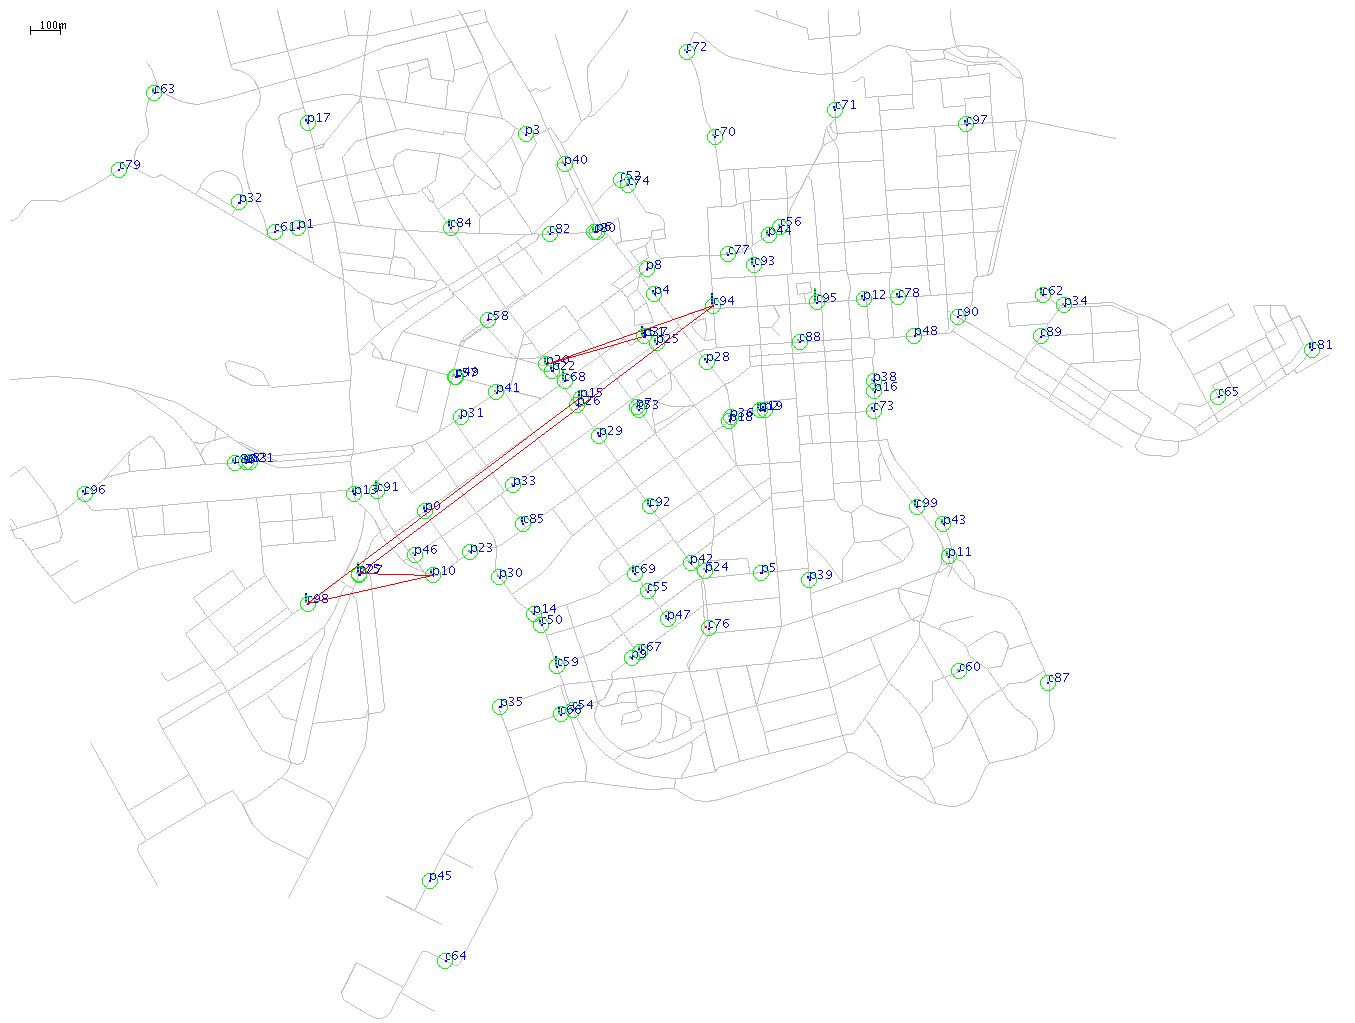
\includegraphics[width=0.5\textwidth]{sixhops.png}
  \label{fig:sixhops}
\end{figure}

Figure \ref{fig:sixhops} shows a multi-hop delivery using the above settings.

\section{Performance Evaluation of the chosen protocols}
\subsection{Buffer Time (Figure \ref{fig:buffertime})}
For all three numbers of hosts the buffer time remains fairly constant for both protocols; with the fewer nodes per group on the network having the lower buffer time.
This is to be expected: fewer nodes on the map means a longer time searching for a node to connect to and send a message to.
In all three numbers of nodes, Prophet gets its messages sent on approximately 50 milliseconds faster than Epidemic; this is somewhat surprising given that Prophet has to perform calculations with respect to probabilities before deciding where a message should go, whereas Epidemic forwards without any such computation.

\begin{figure}[ht]
  \caption{Message size against buffer time for the three numbers of hosts}
  \centering
  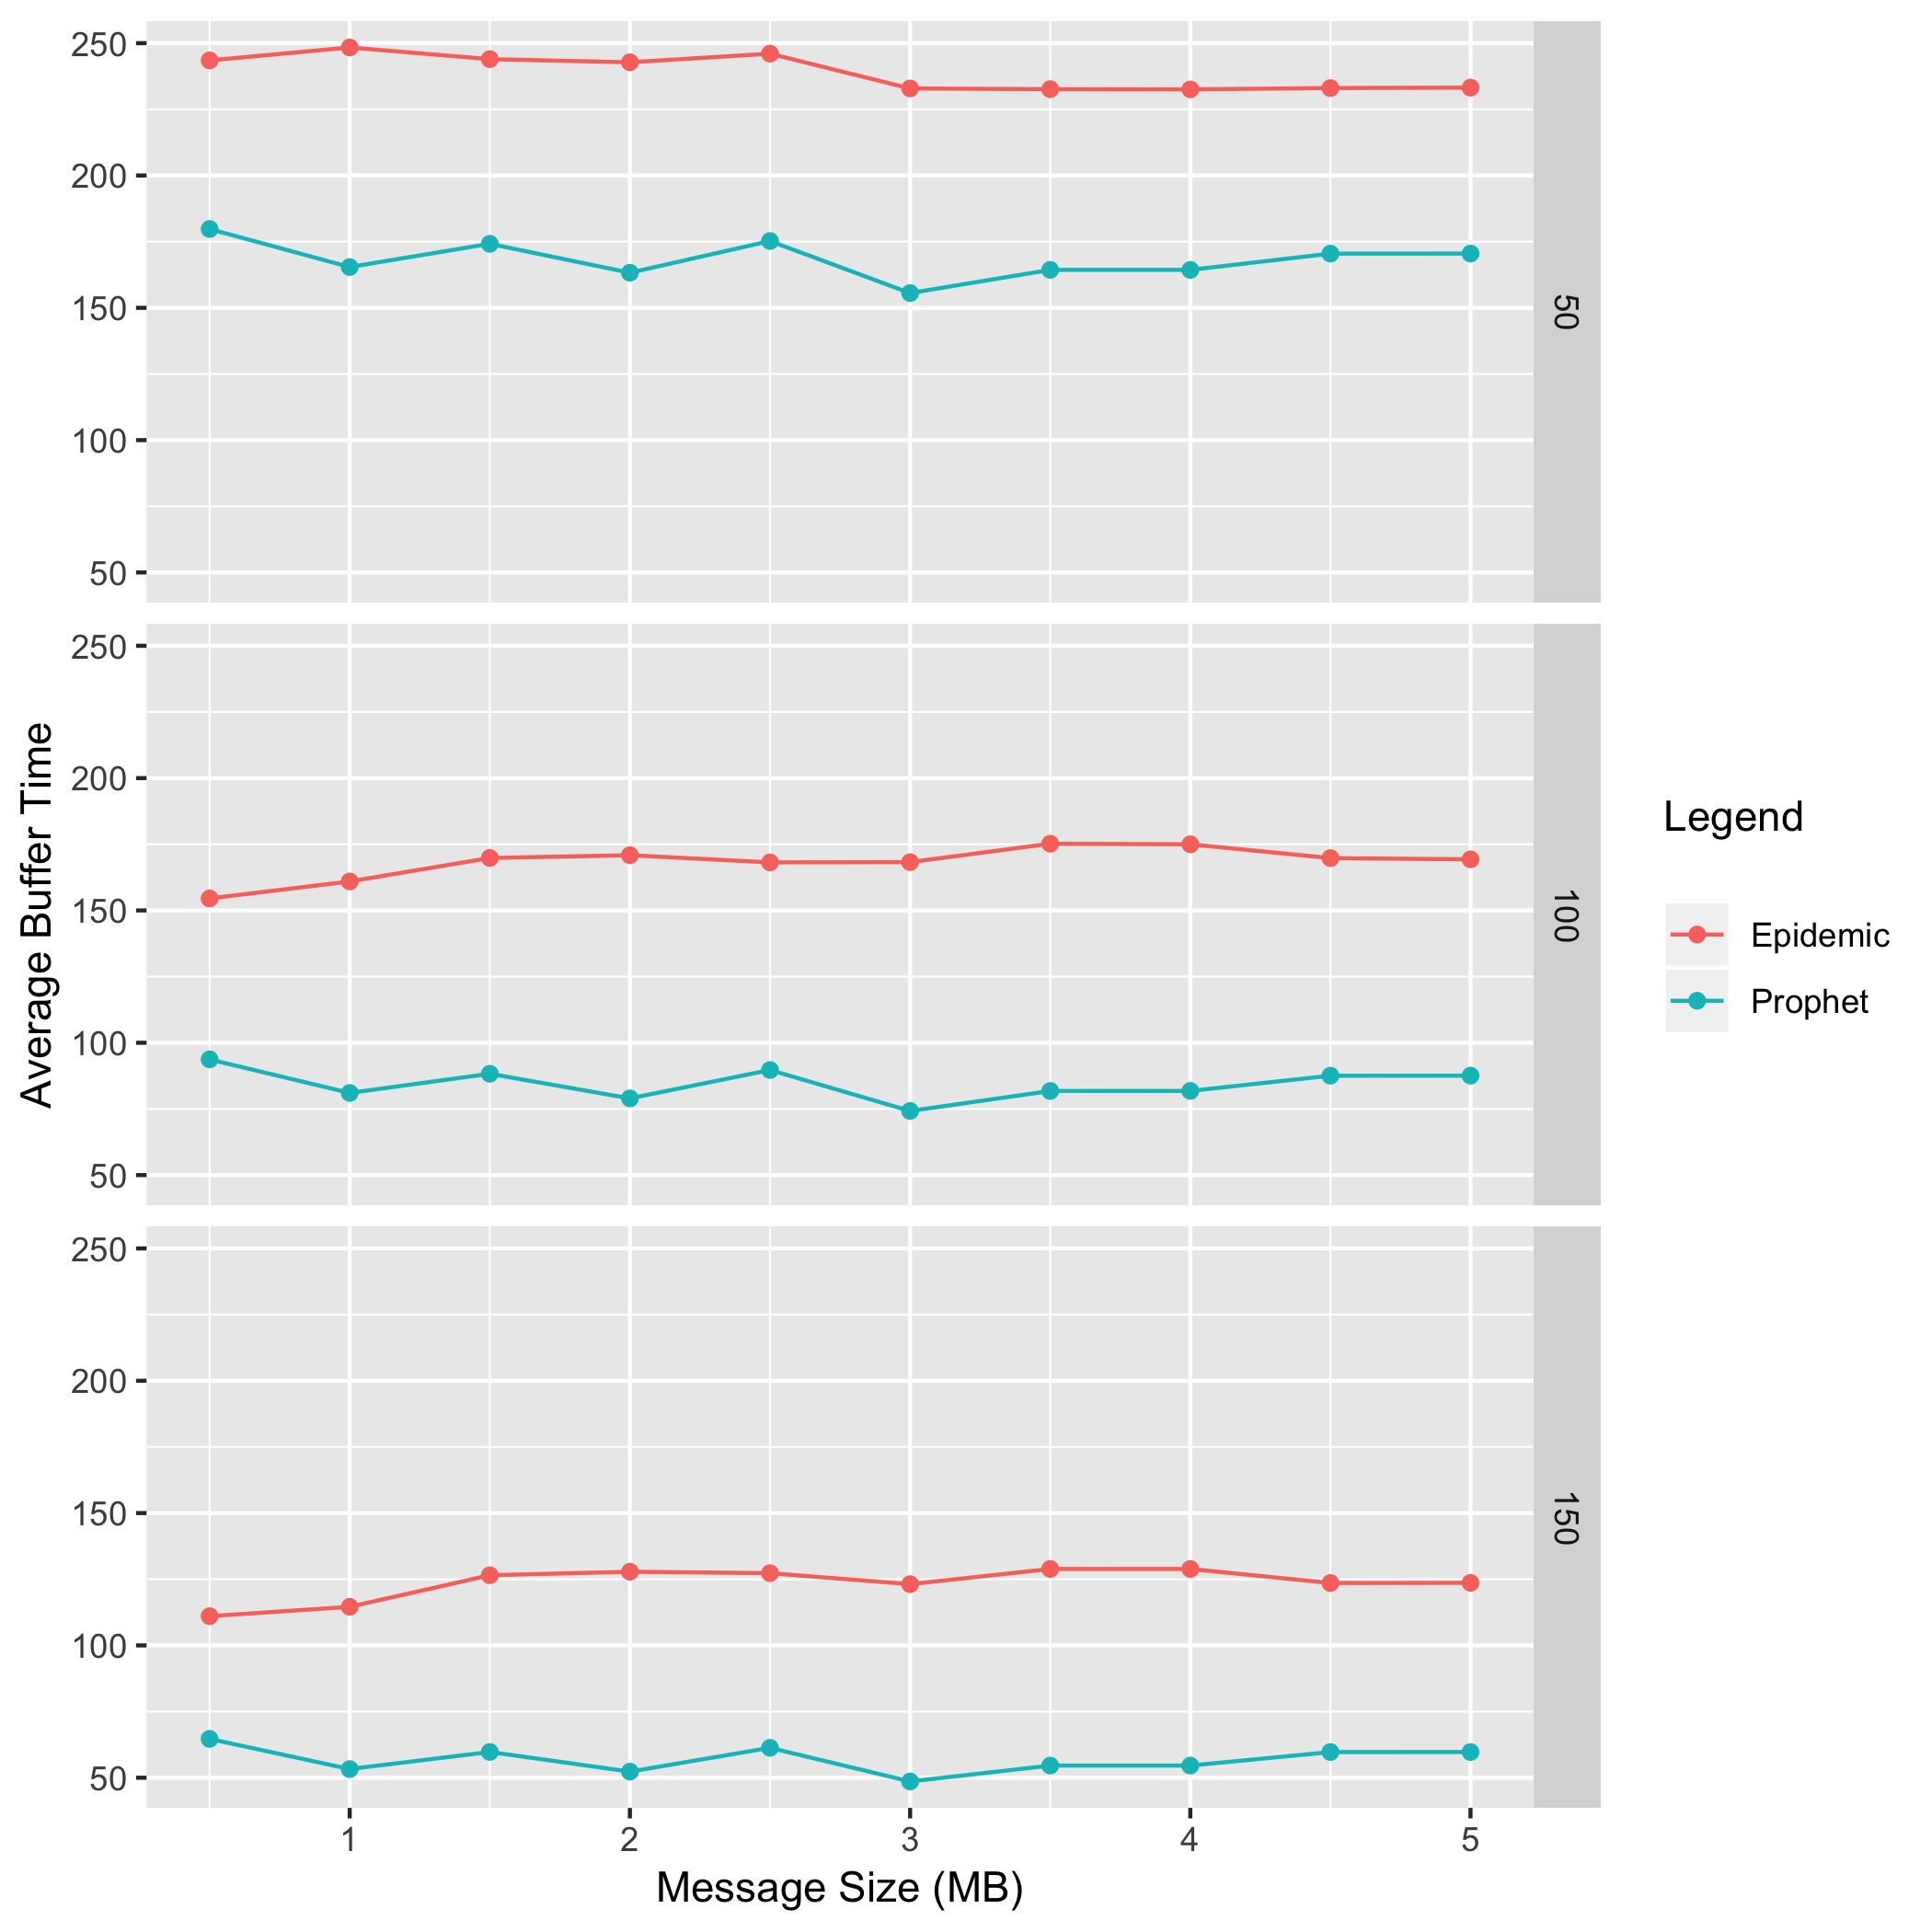
\includegraphics[width=0.5\textwidth]{buffertimeplot.png}
  \label{fig:buffertime}
\end{figure}

\subsection{Hop Count (Figure \ref{fig:hopcount})}
Again unsurprisingly the hop count is smaller the fewer nodes there are; fewer nodes means fewer possible hops.
More interesting is the variance in the number of hops an Epidemic packet takes compared to a Prophet one: Prophet's probability computations are showing their worth here as the most hops a packet takes under it is 8 as compared to Epidemic's maximum of 21.
Indeed this worst case hop number is obtained at low message sizes on the largest number of nodes per group, an understandable outcome which can be attributed to Prophet's "training period" taking longer for such a number of hosts.

\begin{figure}[ht]
  \caption{Message size against hop count for the three numbers of hosts}
  \centering
  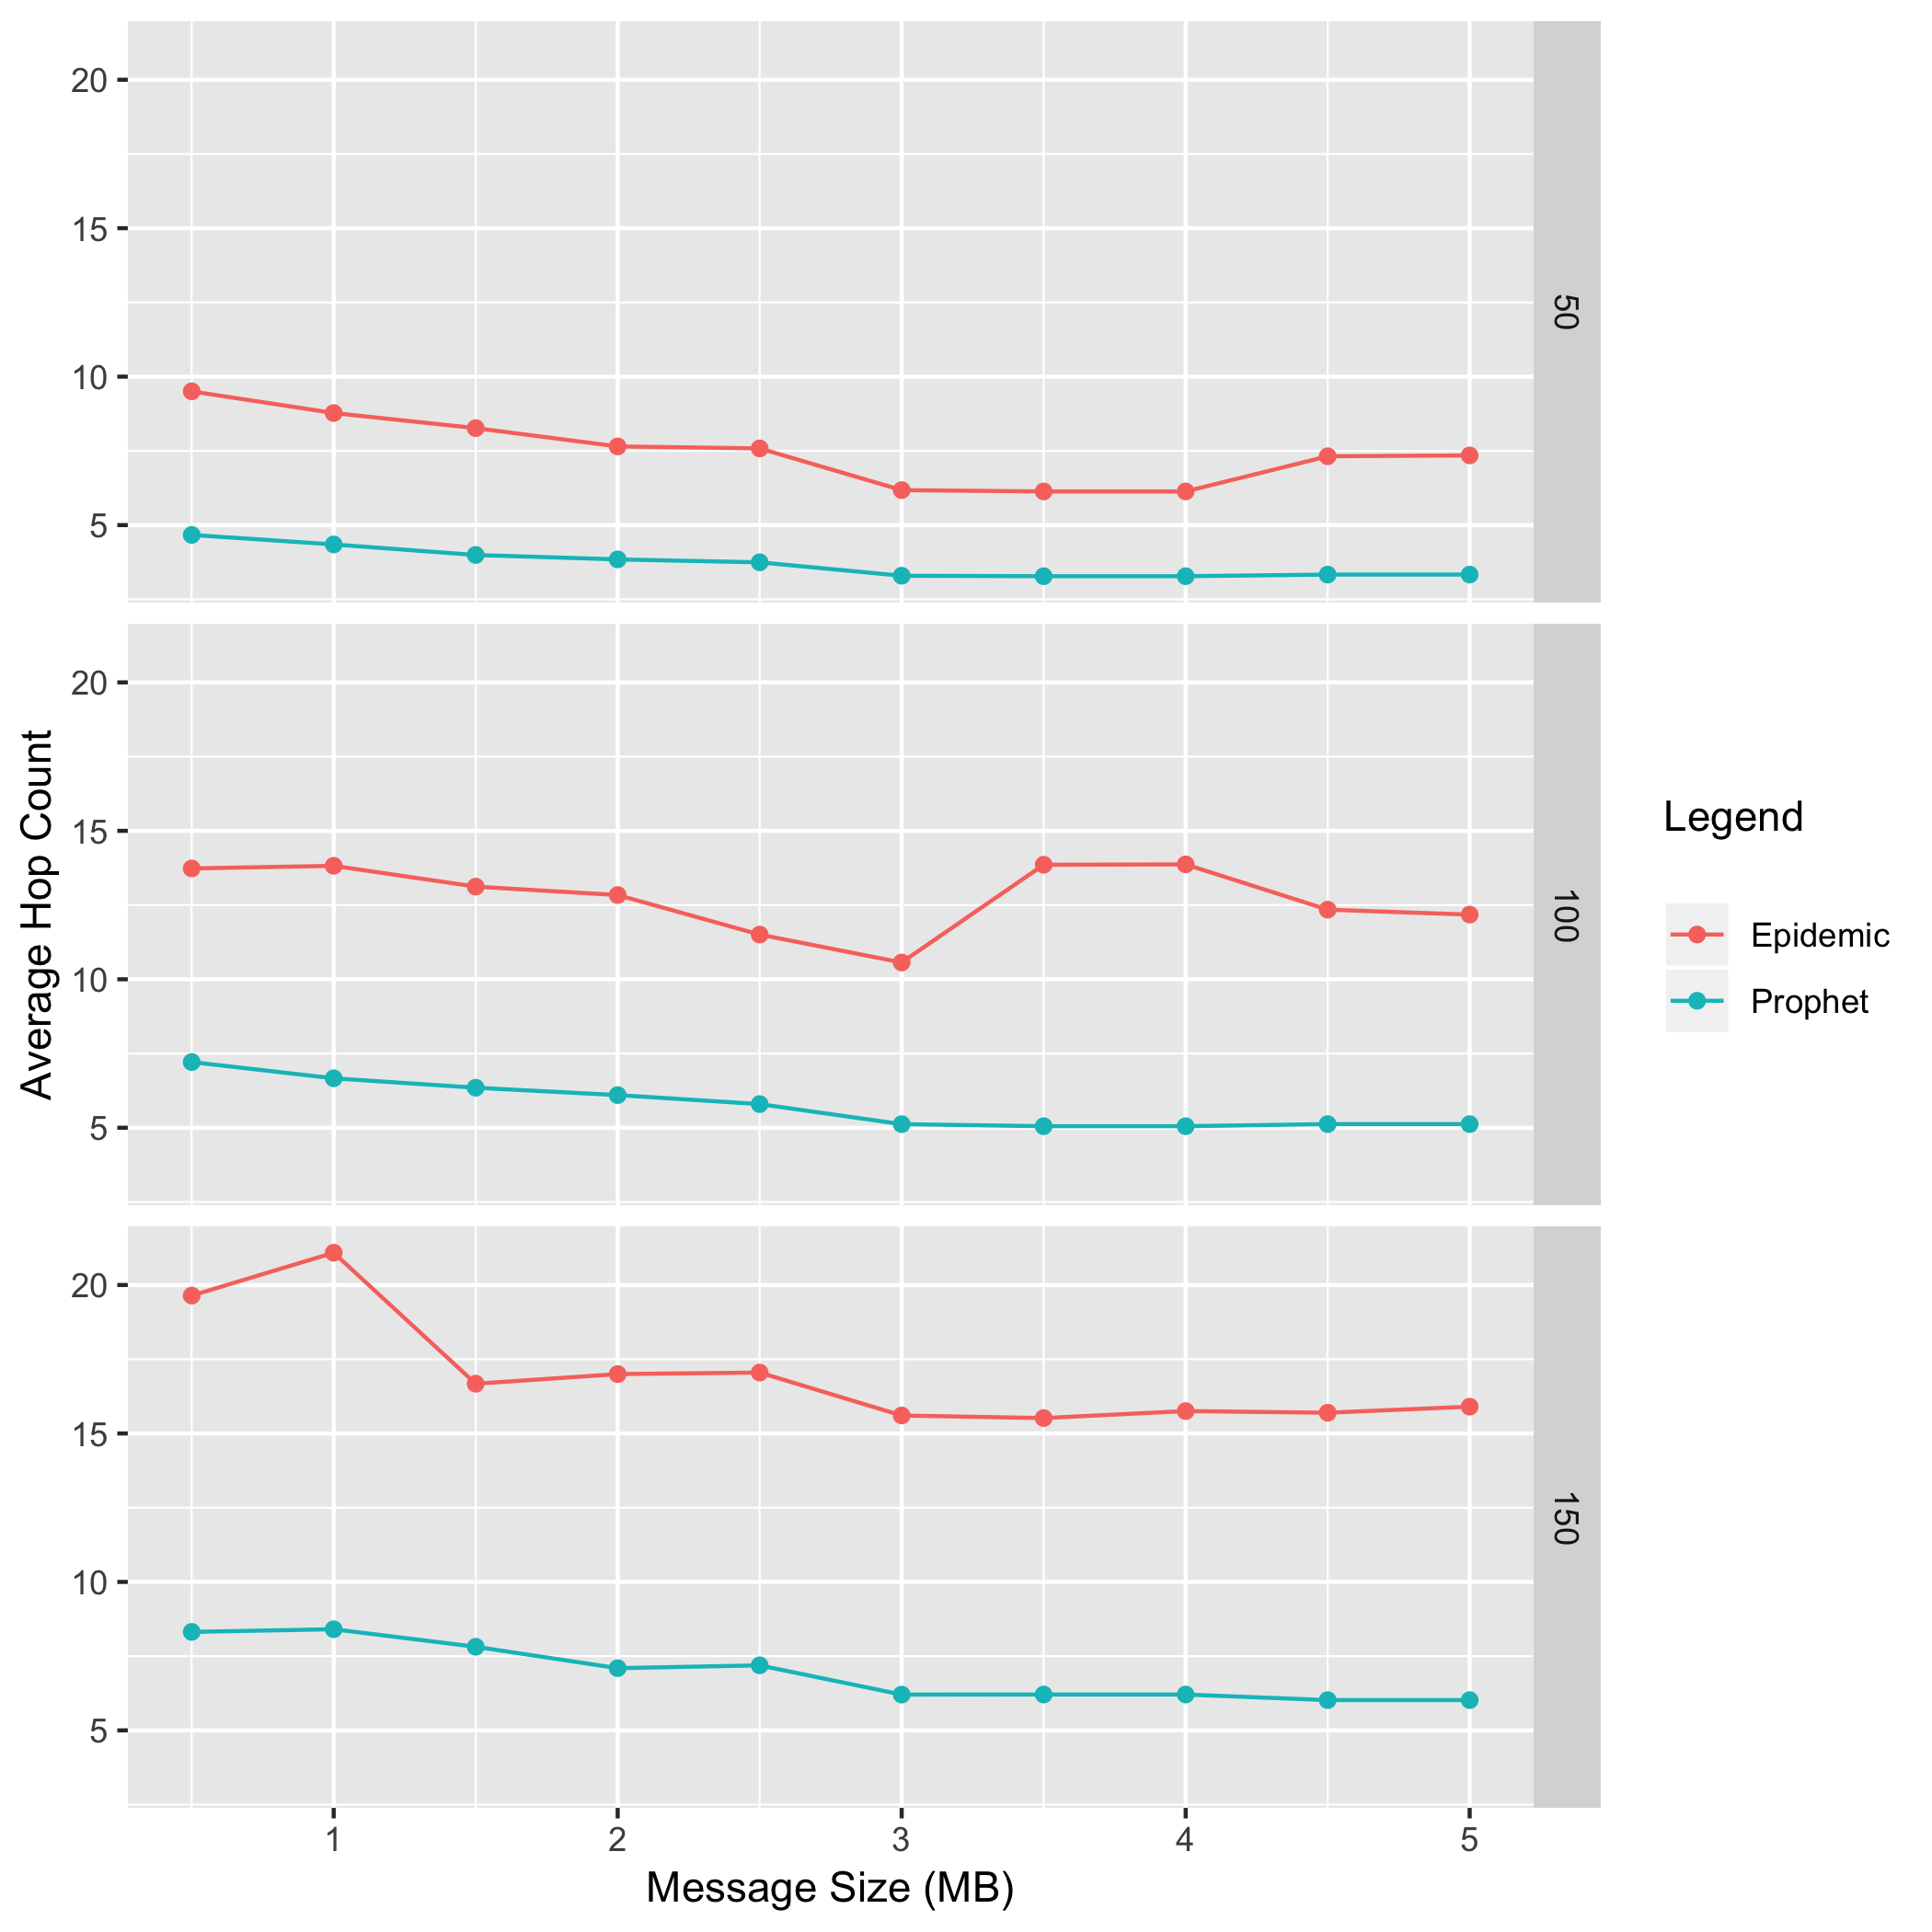
\includegraphics[width=0.5\textwidth]{hopcountplot.png}
  \label{fig:hopcount}
\end{figure}

\subsection{Latency (Figure \ref{fig:latency})}
In general Epidemic "wins" this category, having lower latency almost across the board than Prophet at all three message sizes.
An interesting observation here though is that at Prophet's latency decreases drastically as message size increases until 3MB, whereupon it flattens out.
At all three numbers of nodes per group this latency remains constant, which we can interpret as latency not in fact being related to hop count as a variable.
This is a somewhat strange observation; one would assume (as I have above) that fewer hops would mean a faster-delivered message.
Upon further consideration this is not necessarily the case: fewer hops may mean more time waiting to hop, or a more "considered" hop, which would make up the difference in time by choosing a better route for the packet.

\begin{figure}[ht]
  \caption{Message size against latency for the three numbers of hosts}
  \centering
  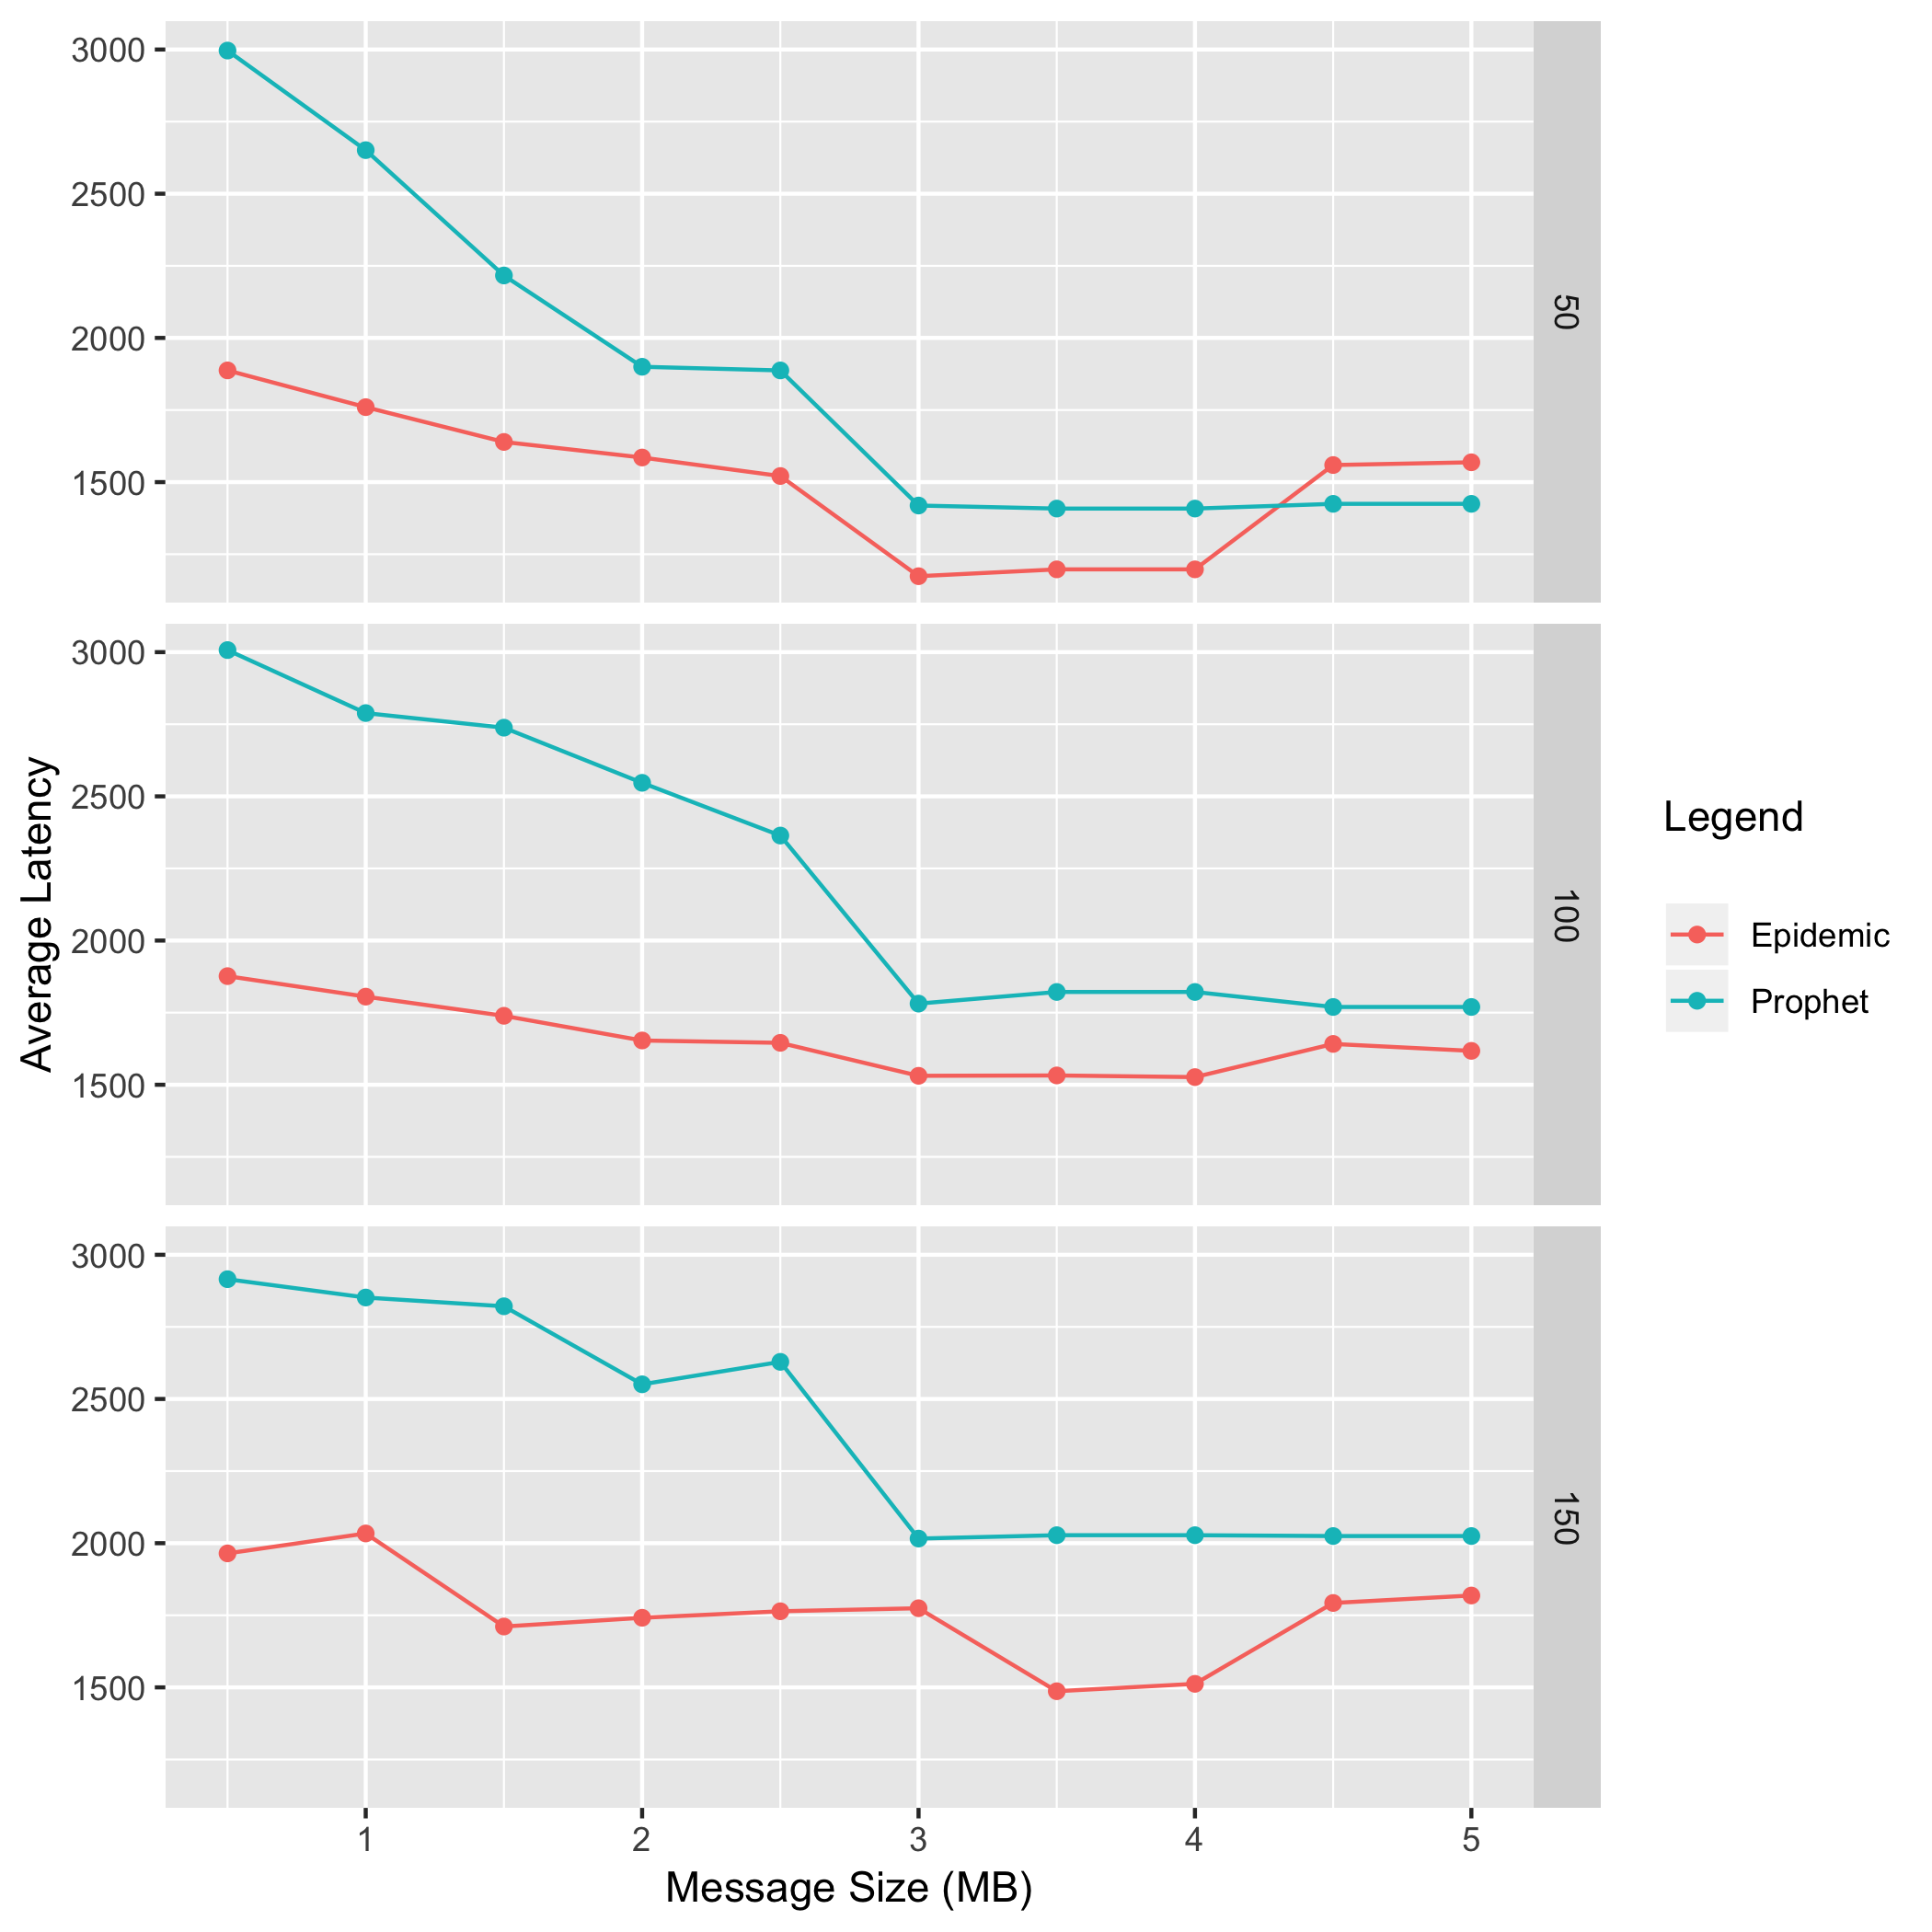
\includegraphics[width=0.5\textwidth]{latencyplot.png}
  \label{fig:latency}
\end{figure}

\subsection{Overhead (Figure \ref{fig:overhead})}
In all three instances the overhead is inversely proportional to the size of the message, in all three instances flattening out at a similar amount past messages of 4MB, but before then the slope is more pronounced the more nodes are present.
Initially this result is interesting because Epidemic, by its nature, does not do much in the way of computations, certainly less than Prophet does with its probability calculations and decision-making.
It is this fact, however, that leads to the higher overhead; all possible destinations have a message sent to them, even those that have no chance of delivering a message.
This leads to more work being done and consequently a higher ovehead.
As well as this, in Prophet's case there is a training period in which the probability is calculated, after which there is considerably less computation involved barring the choosing of who to send a message to (but this is relatively simple in reality), however Epidemic nodes compare every time they wish to exchange a message.
This can be thought of as amortising the overhead, which is to say performing a computationally intensive task once per "cycle" of inputs such that all other operations within that cycle occur substantially quicker compared to a constant series of slightly slower operations.

\begin{figure}[ht]
  \caption{Message size against overhead for the three numbers of hosts}
  \centering
  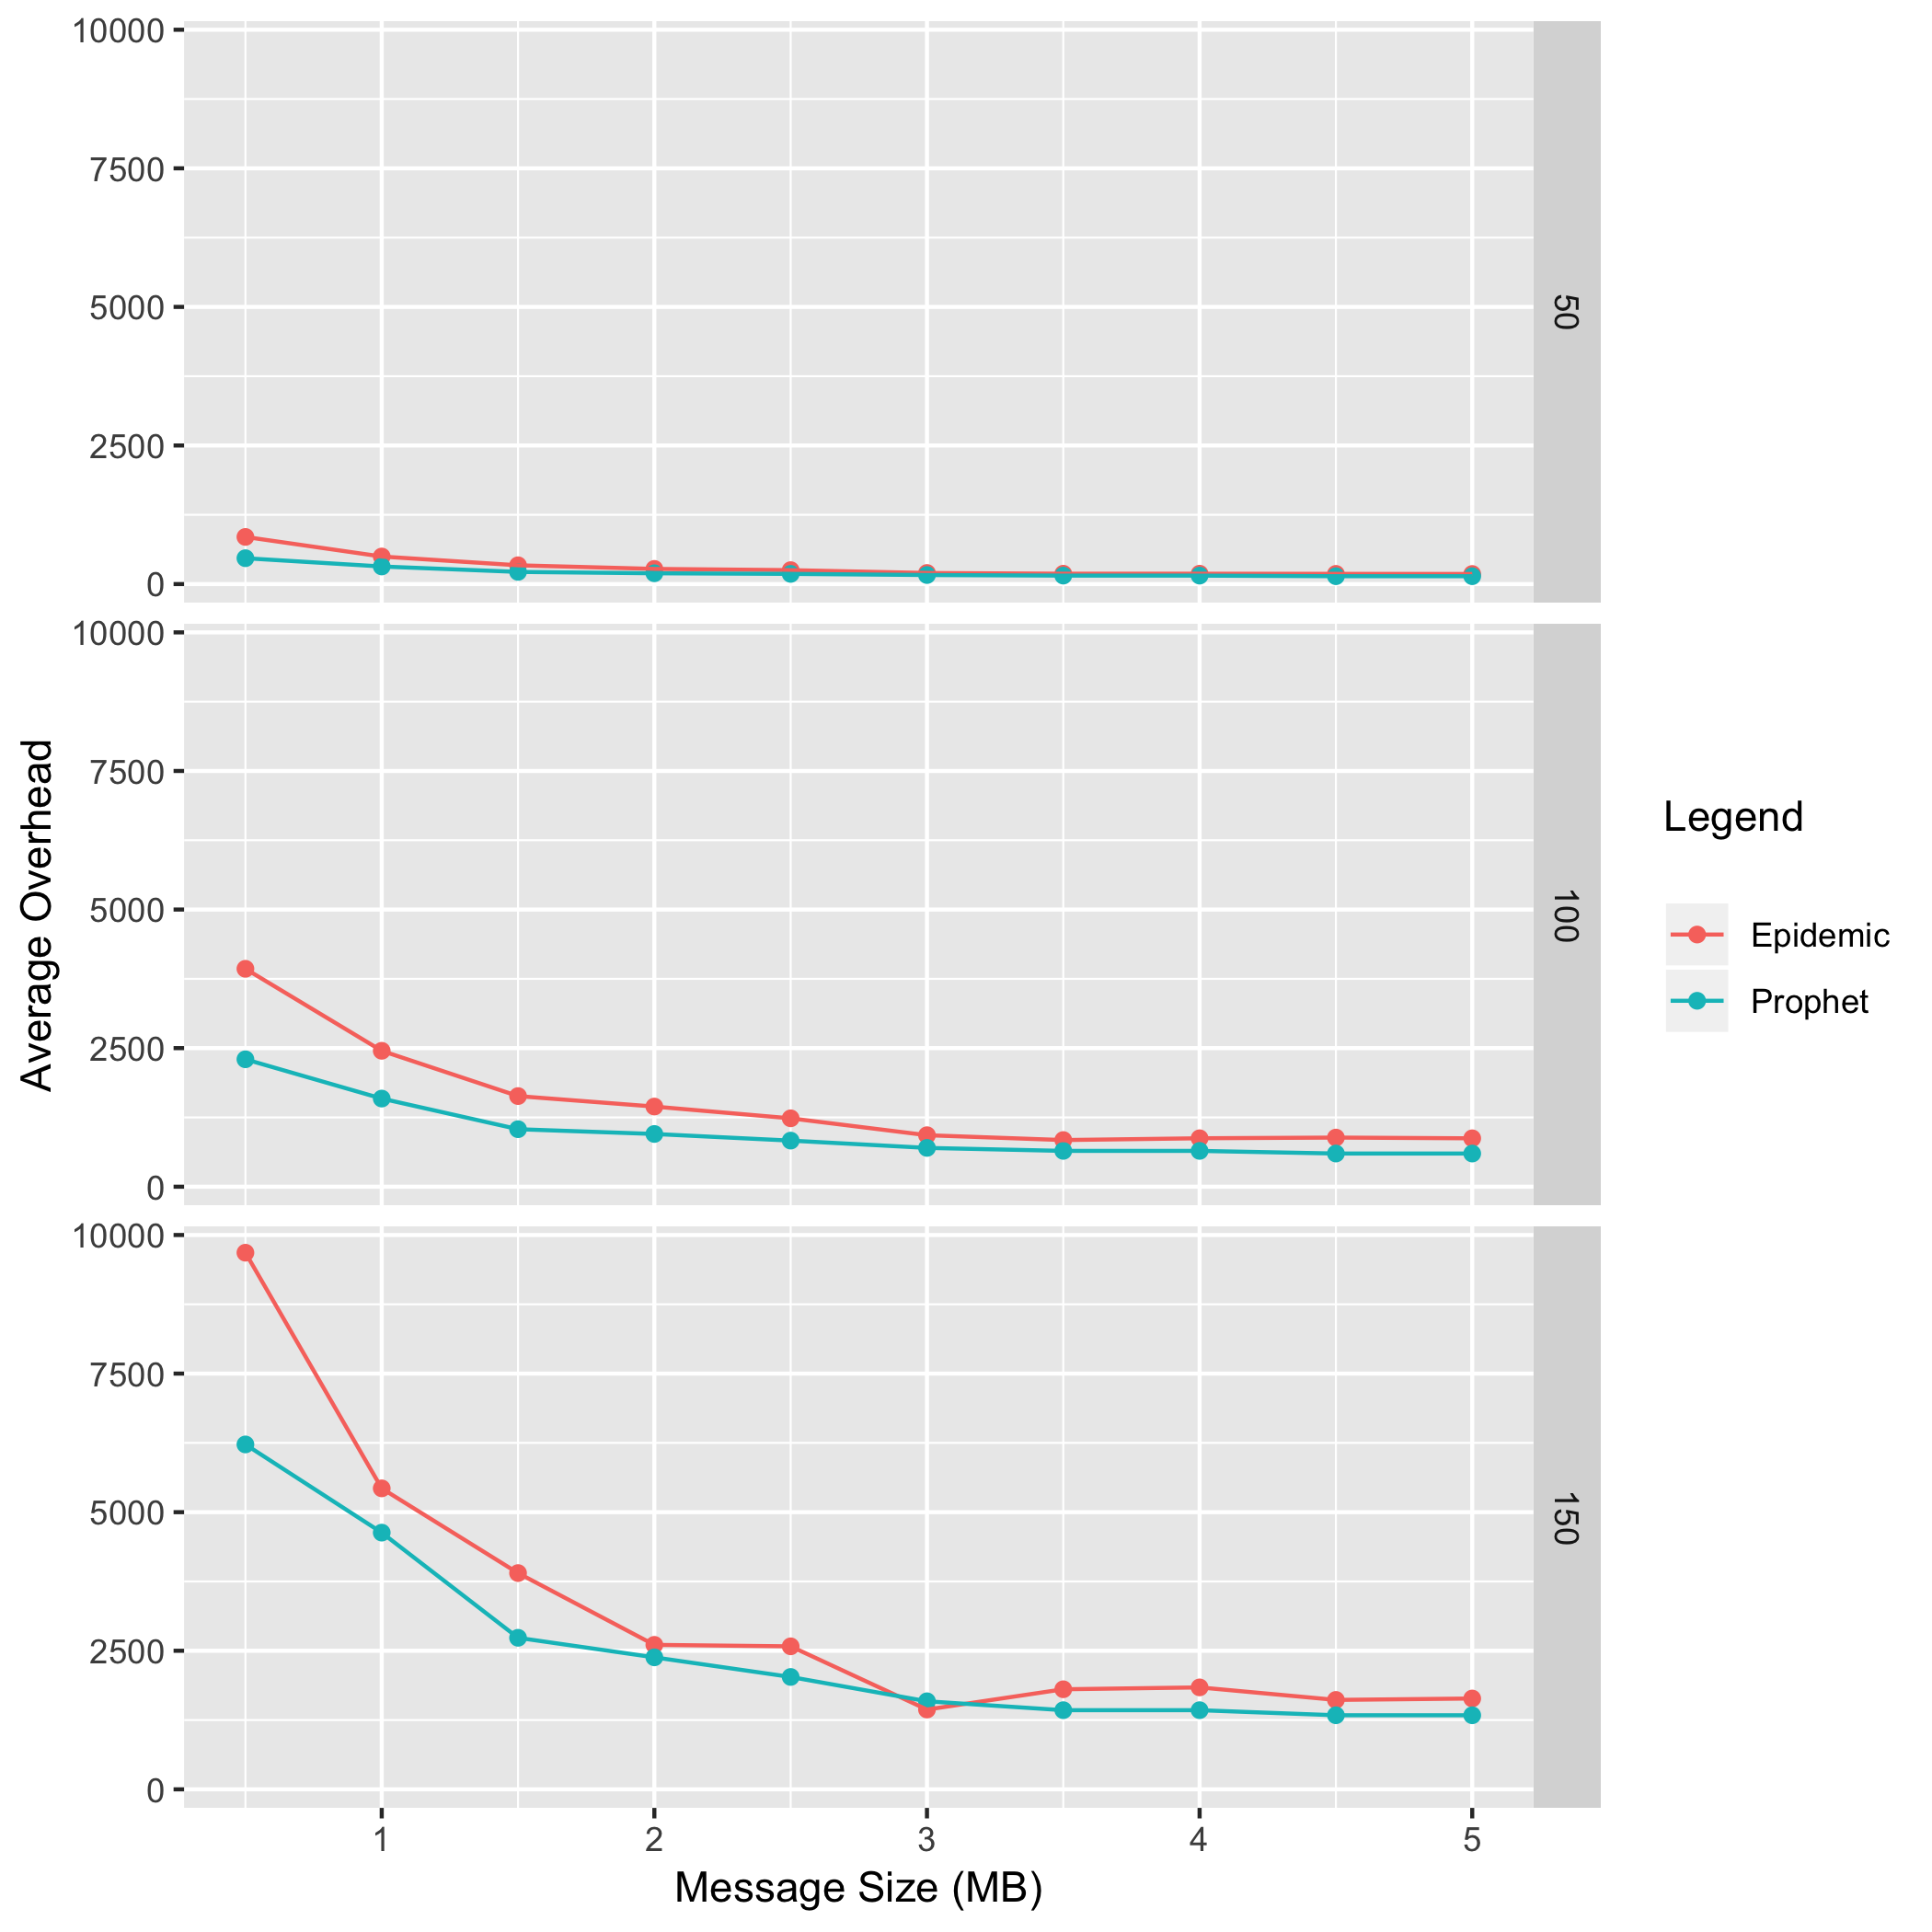
\includegraphics[width=0.5\textwidth]{overheadplot.png}
  \label{fig:overhead}
\end{figure}

\subsection{Delivery Probability (Figure \ref{fig:delivprob})}
By and large a message sent using Prophet has a greater chance of reaching its destination than one sent using Epidemic.
In both cases a smaller message has a greater chance of delivery than a larger one, however with regards to this particular scenario neither can give a delivery success rate above ~30\%.
Interestingly Prophet's delivery probability demonstrates a considerably shallower, more constant slope than Epidemic's, both displaying a small "spike" at messages of 2.5MB.
It is unclear as to where this spike comes from, however at 3MB the probability goes down after which it actually increases up to 5MB messages.

\begin{figure}[ht]
  \caption{Message size against delivery probability for the three numbers of hosts}
  \centering
  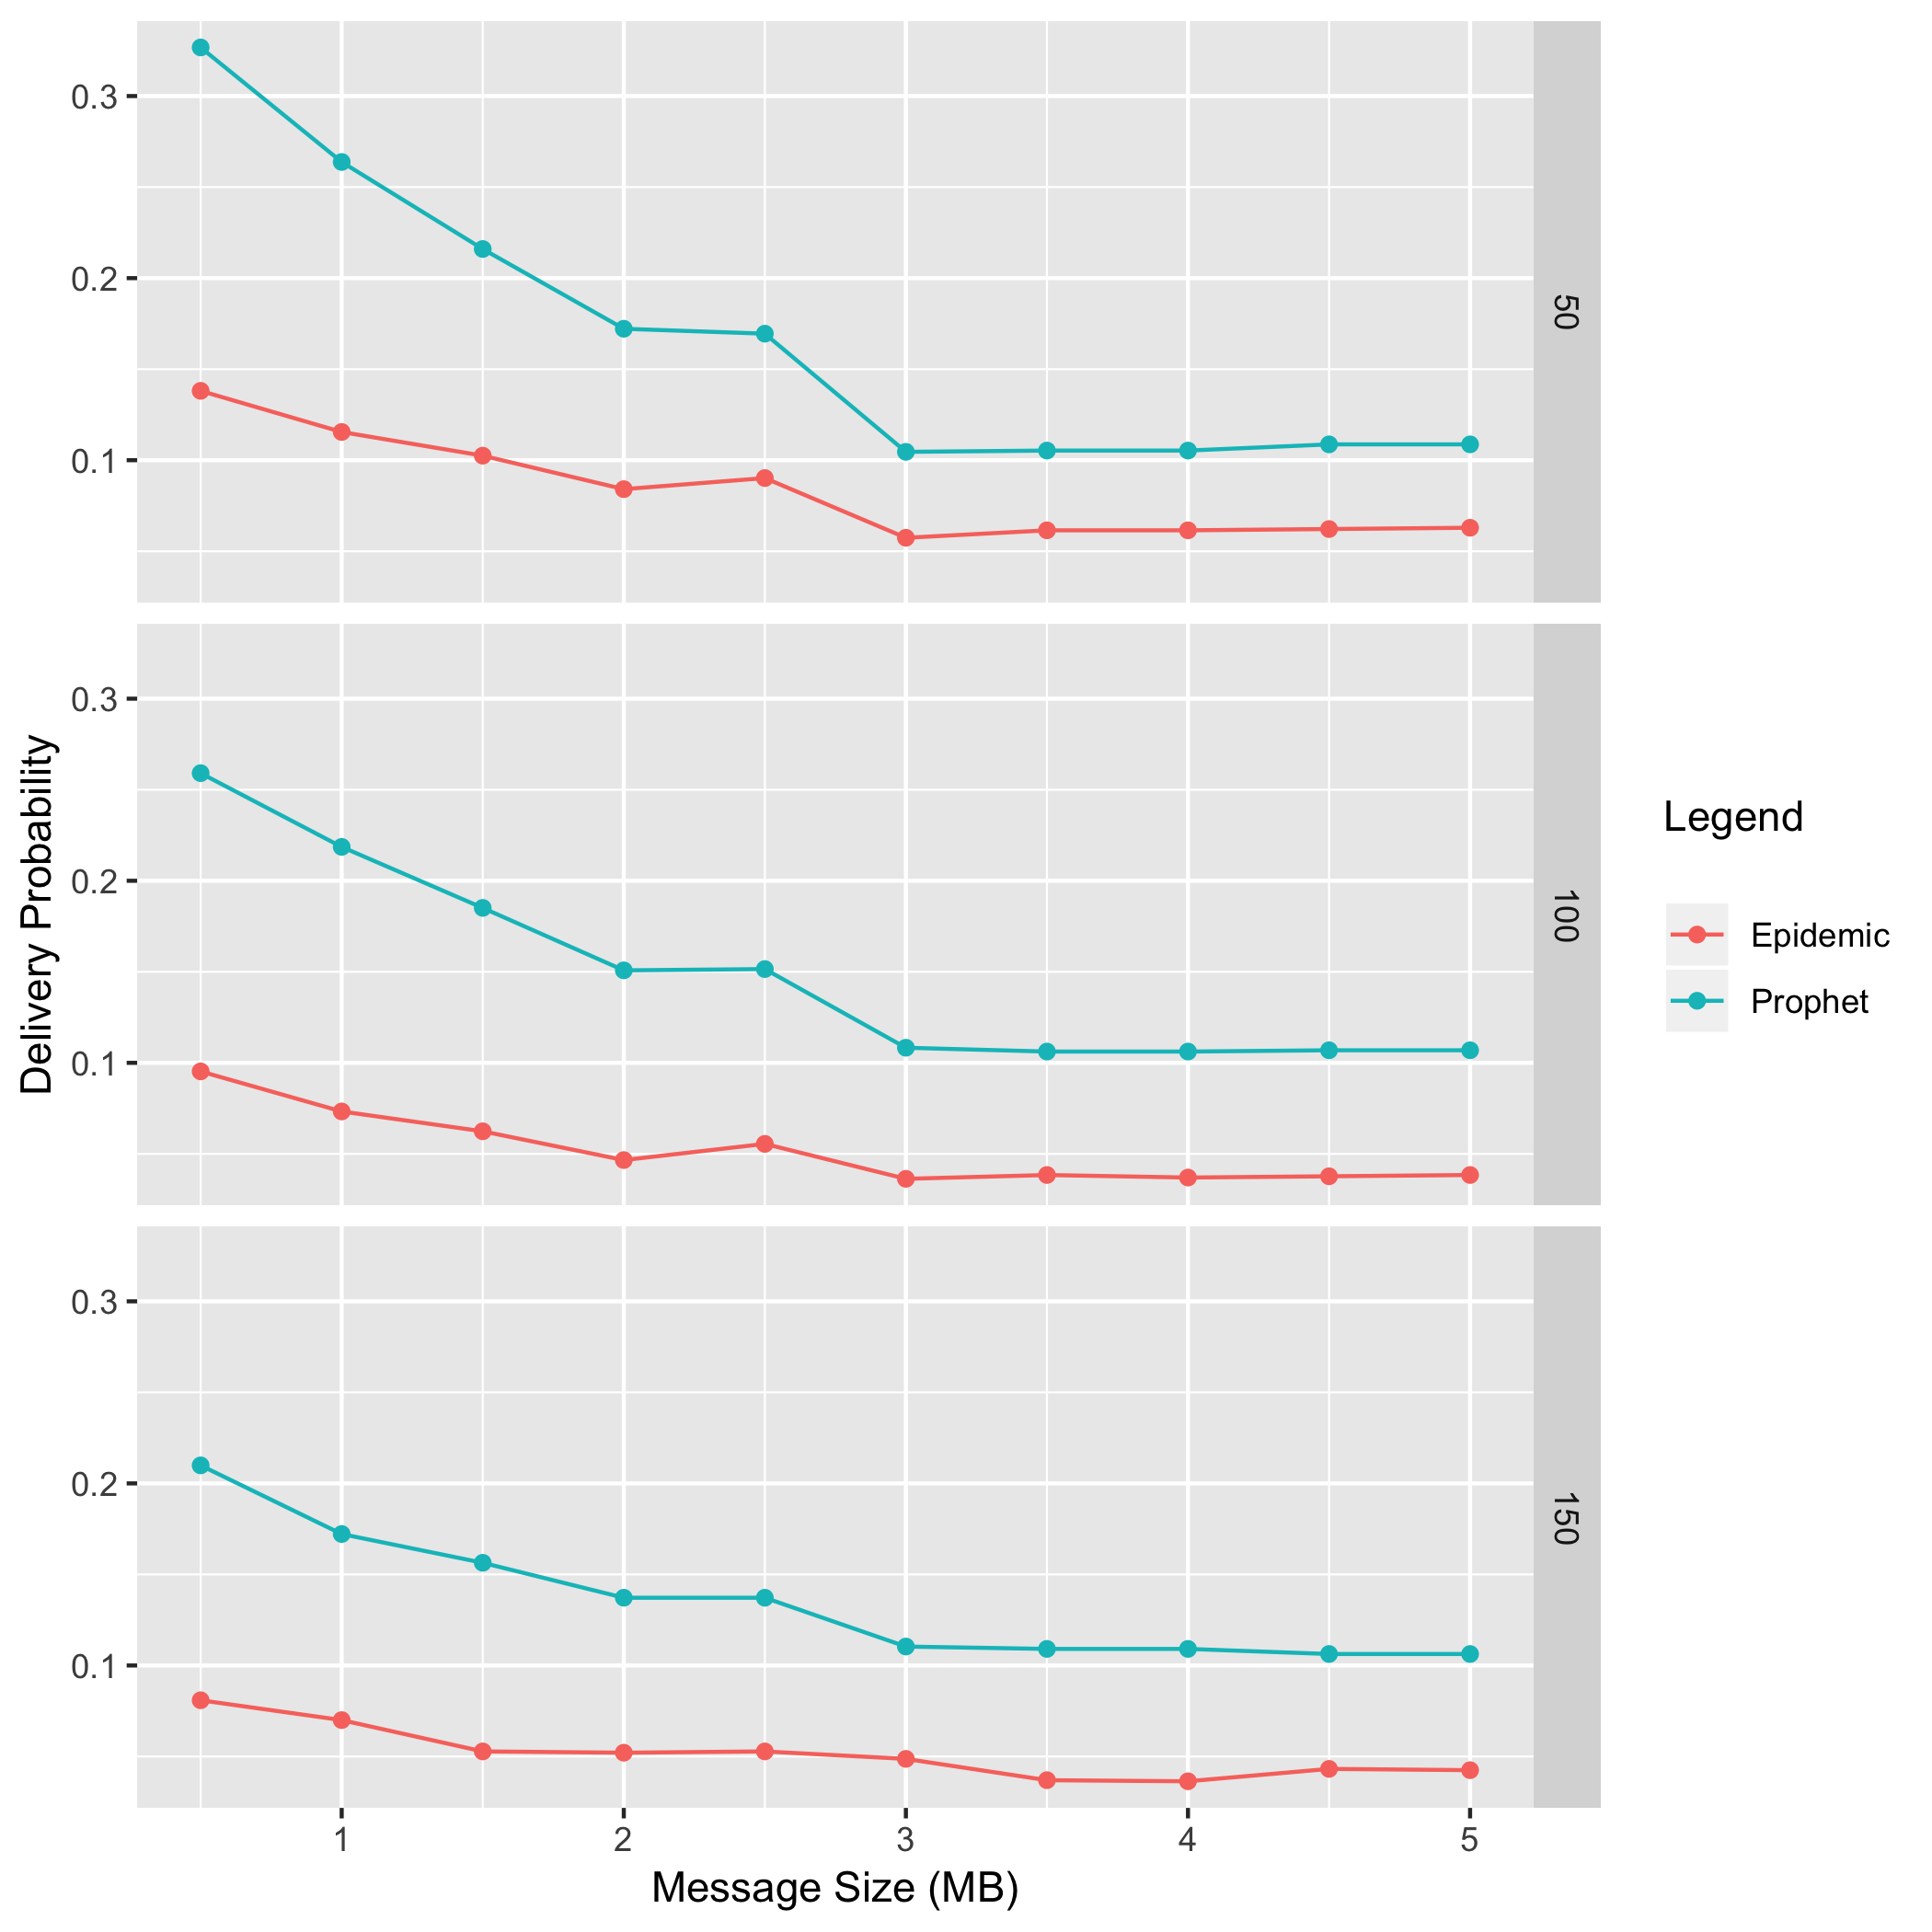
\includegraphics[width=0.5\textwidth]{delivprobplot.png}
  \label{fig:delivprob}
\end{figure}

\subsection{Conclusion of Comparisons}
Based on the information gathered I believe that in most cases it is advisable to use Prophet over Epidemic for this situation (unless minimum latency is the absolute goal).
It performs better in buffer time, hop count, overhead, and delivery probability (which realistically is the end goal of a MANET algorithm: to deliver a message from point A to point B without a structured/constant network).
Indeed, even in the case of latency, Prophet, at messages 3MB and above, is consistently only 25\% worse for this metric (even being better at higher message sizes for 50 hosts).

\section{Discussing the pros and cons of Opportunistic Networks}
Based on the results of the experiments above, it appears that opportunistic networks are somewhat unsuitable for the above scenario.
The fact that neither protocol can reliably deliver above 30 \% of messages suggests that they are ultimately not worth using.
This is, however, in my view a naive outlook; in such a scenario any protocol that requires a permanent, fixed connection will not be able to deliver messages whatsoever, and consequently any system that allows for such delivery is an improvement and therefore suitable for the scenario.
It is likely though that other protocols may perform better on a success rate basis.

\par

In disaster settings in general Opportunistic Networks are hugely suitable as means of quickly establishing communications systems where more traditional protocols would be "knocked out" by the disaster.

\par

Other settings too can benefit hugely from more advanced Opportunistic Network technologies; driverless cars are a field being increasingly explored, DARPA's Grand Challenge in 2004 offering \$1000000 to a team whose autonomous vehicle could travel 150mi through the Mojave Desert in California\cite{darpachallenge}.
Opportunistic Networks could be used to great effect in this field, with each vehicle as a node on the VANET they could pass information between each other about difficult terrain, nearby accidents, or routes to avoid.
Again though if the experiments run above are to be believed, such network protocols require a great deal of work to become fully useful; when life and limb are at stake a 30\% success rate is not good enough.
Additionally to this security will become a major issue, with Opportunistic Networks being so trusting of new nodes joining a malicious user could connect to the VANET, release either a malicious packet designed to disable vehicles, or even simply misinformation that could lead to injury.
This security issue is something that will require a great deal of work to overcome, with any kind of network authentication leading to more overhead and more resources being required.

\begin{thebibliography}{0}
  \bibitem{ieeemag}
    Opportunistic Networking: Data Forwarding in Disconnected Mobile Ad Hoc Networks\\
    IEEE Communications Magazine, November 2006, pages 134-141\\
    Pelusi, Passarella, Conti
  \bibitem{onewebsite}
    The ONE (ONE Official Website)\\
    https://akeranen.github.io/the-one\\
    Accessed 2018-10-08
  \bibitem{epidemicreport}      % INTRODUCES EPIDEMIC
    Epidemic Routing for Partially-Connected Ad Hoc Networks\\
    Amin Vahdat and David Becker\\
    2000
  \bibitem{prophetreport1}      % INTRODUCES PROPHET
    Evaluating opportunistic networks in disaster scenarios\\
    A. Martin-Campillo, J. Crowcroft, E. Yoneki, and R. Marti\\
    2013
  \bibitem{simutools}
    Kerãnen A, Ott J, and Kãrkkãinen T\\
    The ONE Simulator for DTN Protocol Evaluation\\
    In SIMUTools ’09: Proceedings of the 2nd International Conference on Simulation Tools and Techniques\\
    New York, NY, USA\\
    2009
  \bibitem{darpachallenge}
    Darpa Grand Challenge 2004 DARPA's Debacle in the Desert\\
    \textit{Popular Science}\\
    Published 2004-06-04\\
    Accessed 2018-12-07\\
    www.popsci.com/scitech/article/2004-06/darpa-grand-challenge-2004darpas-debacle-desert
  \bibitem{vaccines}
    Zhang X, Neglia G, Kurose J, and Don Towsley D.\\
    Performance modeling of epidemic routing\\
    \textit{Computer Networks}\\
    2005\\
    Accessed 2018-12-07
\end{thebibliography}

\end{document}

